\section{Introduction}
\label{sec:intro}

The development of the Internet has spawned a number of task-oriented writings, such as product descriptions on Amazon. However, since writers cannot always have a thorough understanding of consumers' need, their writings usually miss something deemed important by audience. For example, an American writer may assume his machine be used on 110V and thus omit this in description, while customers from other countries may requires it to work on 220V. Discussion areas like Amazon's Customer QA were established for users to ask for those missing information. So we may ask ``What is the voltage of this machine?" for the previous example. However, such user engagement can not be achieved for new products or platforms.

\begin{figure}[htbp]
\centering
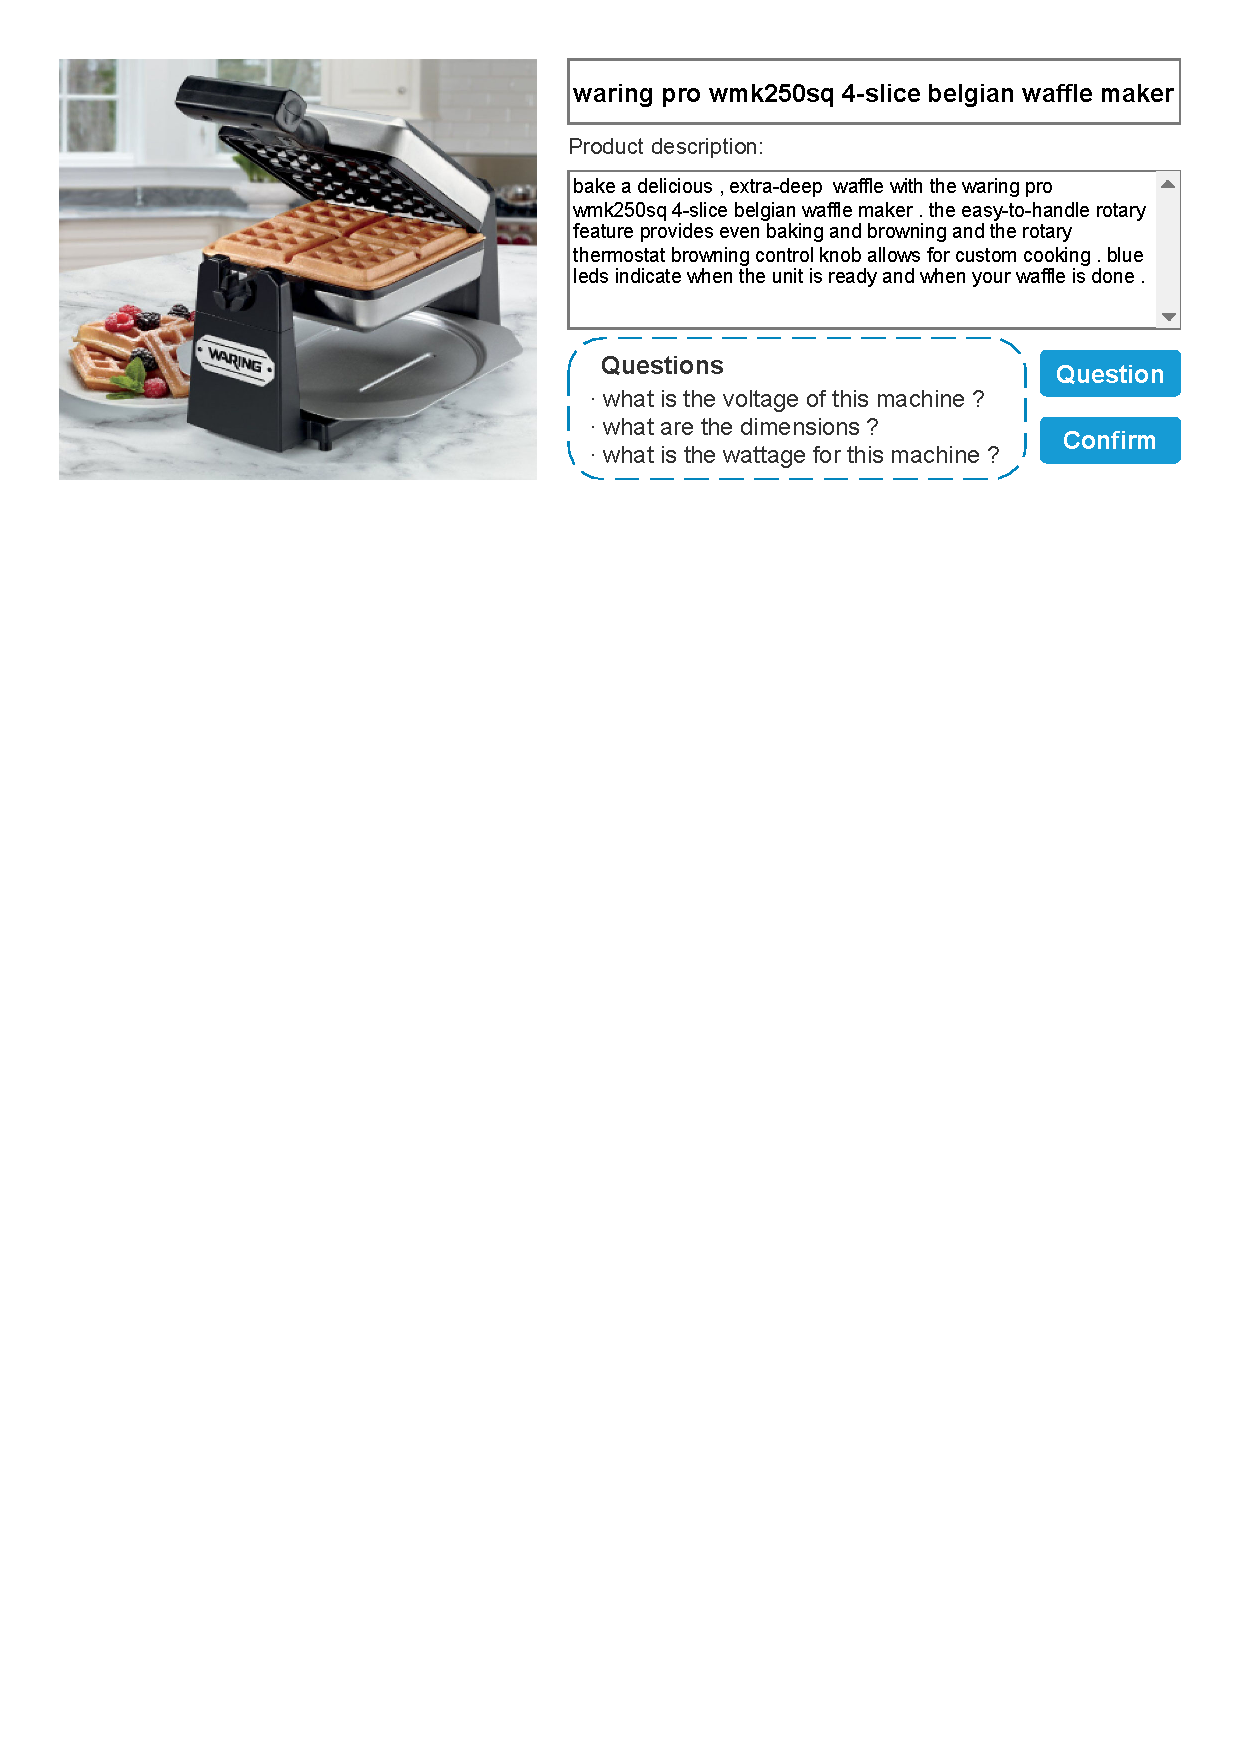
\includegraphics[width=\linewidth]{WA_UI.pdf}
\caption{UI of the writing assistant.}
\label{fig:WA_UI}
\end{figure}

Clarification question\footnote{questions asking for what's missing from a given context} generation (CQGen) is a promising approach that mimics the user engagement to help task-oriented writings. Pioneering works like \citet{rao2019answer} have proposed sequence-to-sequence (seq2seq) models to tackle the theoretical task. However, to our best knowledge, no prior work has considered practical scenario for this technique. 
% \KZ{Rephrase this: This is fundamental for researches on this task, because we can't make proper evaluation on the algorithm unless we know how it will be used.} 
% \Zl{Does seem strange in the context, removed it.}
% \KZ{This so-called ``design'' still seems quite naive to me. Yet you spend a long paragraph on it. Maybe say: consider the following scenario, ...blah}
Therefore, we consider one possibility: a writing assistant. Figure \ref{fig:WA_UI} shows an example for e-commerce scenario. To publish a product, the vendor first enters the title and description of the product as the basic context. Then he/she can press the ``Question" button, and several CQs will be shown at the ``Questions" panel, helping the vendor to supplement possibly missing information. The vendor can press ``Confirm" to publish the product when confident enough, or he/she can press ``Question" for a different set of questions so as to iteratively improve the writing. 

Note that the system will show a group of questions instead of one, as is assumed in traditional experimental settings, because this design allows the system to efficiently cover a variety of user needs at one time, and will be more robust to problems on any single generation. This raised the demand for \textit{diversity} with in a generation group. We thus seek CQGen algorithms that can meet the requirement, and adopt a new group-level evaluation protocol to properly evaluate the system performance under this scenario.

CQGen is a challenging task. First, it requires the question to be \textit{specific} while not being \textit{repetitive} to existing context. Vanilla seq2seq model has been shown to generate highly generic questions by \citet{rao2019answer}. They then proposed GAN-Utility for this problem. However, their approach requires another QA component to generate answer from context and the generated question, which may not be reliable as the answers are inherently missing from context by definition. Consequently, this approach was shown to yield even worse result under some conditions \citep{cao2019controlling}. Moreover, we need to generate a group of diverse questions here. This challenge is first tackled along with our proposal of writing assistant. 

To deal with the specificity challenge, we propose a novel model named Keyword Prediction and Conditioning Network (KPCNet). We observed that the main semantics of a question can be captured by its keywords. For example, the keyword of ``What's the \textit{dimension}?" is \textit{dimension}, and the question can be comprehended even with a single word (``\textit{dimension}?"). Keywords mainly consist of the product properties, and can allow for even more flexible and specific generation sometimes. For example, we can generate ``Can you cook \textit{rice} in this \textit{cooker}?" with keywords ``\textit{cooker, rice}", while it will be unsuitable to use properties to exhaust all possible ingredients like \textit{rice}. Therefore, the proposed KPCNet first predicts the probability for a keyword to appear in the generated CQ, then selects keywords from the predicted distribution, and finally conditions on them to generate questions. We also found that we can partially control the generation by operating on the conditioned keywords, which can be utilized to avoid repetitive questions and further improve the quality.

To promote diversity, we explore several diverse generation approaches for this problem, including model-based \textit{Mixture of Experts} \citep{shen2019mixture} and decoding-based \textit{Diverse Beam Search} \citep{vijayakumar2018diverse}. KPCNet's controllability through keywords also allows keywords-based approaches. We thus propose a clustering method for keyword selection to generate correct, specific and diverse questions with coherent keyword groups.
% \KZ{Do you really want them to be completely disjoint?
% How about \{cooker, rice\} and \{cooker, soup\}?}.

% \Zl{Partially overlapping is expected. However, overlapping clustering algorithms are usually 'soft' and thus hard to operate. For example, this can be achieved using LDA, with words' prob distribution over topic as its affliation to the cluster. To get a hard membership, we have to tune a threshold. Therefore, I'm currently using disjoint clustering algorithm. By the way, I removed disjoint here.}

Individual and group-level evaluation showed that KPCNet is capable to produce more diverse and specific questions than competitive baselines, and can thus serve as a reliable backbone of the proposed writing assistant. Our contributions are:

\begin{enumerate}
  \item We propose KPCNet, which first predicts keywords for specificity, and then selects keywords as condition for generation to allow partially controllable generation.
  \item Based on the controllability of KPCNet, we propose several selection methods for conditioning keyword sets to promote diversity.
  \item We evaluate KPCNet on 2 datasets (\texttt{Home \& Kitchen} and \texttt{Office}) at both individual-level and group-level. A combination of automatic and human evaluation shows that KPCNet can achieve superior specificity in both settings and outperform strong baselines in diversity.
\end{enumerate}
